\chapter{Technical and Legal Background}

\section{Browser Extensions}
We implemented CookieAudit as a browser extension.
To understand the implementation details in \cref{ch:implementation}, we will give an overview about the architecture and implementation of browser extensions.

Browser extensions are programs that can extend and change the functionality of browsers.
They are built using web technologies (JavaScript, HTML, CSS) and can use APIs provided by the browser.
The browser APIs of Chromium based browsers (e.g., Chrome and Edge) overlap in large parts with the APIs of Mozilla's Firefox and Apple's Safari.
This means that many extensions can run in all those environments.

We have developed CookieAudit according to Manifest version 3, which is the newest specification of the extensions API for Chromium browsers.

When building browser extensions, developers have to split up their code in a pre-defined way.
The JavaScript code that contains the general extension business logic and is not tied to specific web pages, is packaged in the \emph{Extension Service Worker}


\begin{figure}
	\centering
	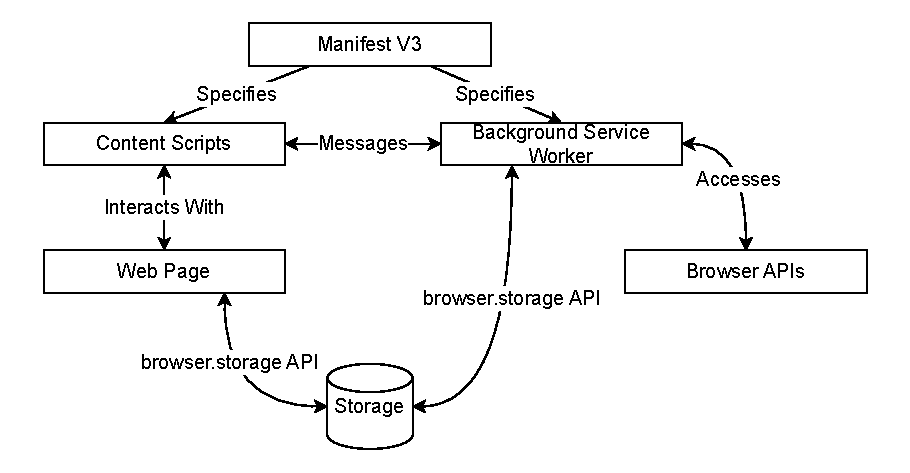
\includegraphics[width=\textwidth]{media/browser-extension-architecture.drawio.pdf}
    \caption{The general architecture of a manifest version 3 browser extension.}
    \label{fig:extension-architecture}
\end{figure}